%%% Local Variables:
%%% mode: latex
%%% TeX-master: "../report"
%%% End:

%%% TODO: move this to kite design
Functional languages often make extensive use of lists, which is indeed also the case for Kite. A list is an ordered array of items that can be transformed in many different ways. We use a common short-hand method for describing a list of things, using square brackets $[\ ]$. For instance, a $List(Int)$ (pronounced ``List of Ints'') is denoted $[Int]$ and a list of a type variables $a$ is $[a]$. Lists can be nested, allowing $List(List(Int))$ denoted $[[Int]]$.

The pair type is also abbreviated using $(,)$, for instance the type $Pair(Int, Bool)$ is written $(Int, Bool)$
%%%

To describe the overall design of the Kite compiler, we will start by
breaking it down into general parts, where each part or module has a
specific task. Below we have a waterfall model including the main
parts of the compiler:

\begin{figure}[H]
  \label{fig:flow}
  \center
  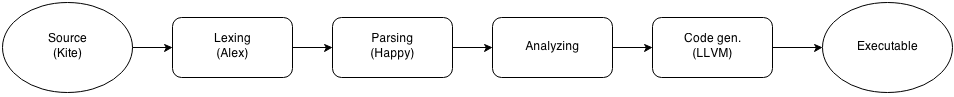
\includegraphics[scale=0.45]{images/flow.png}
  \caption{General flow of the Kite compiler}
\end{figure}

At first it can seem a little daunting, but when we get into the
purpose of each step, there will be a more obvious flow.

\subsection{Preprocessor}
The first thing the compiler does is preprocess the input, e.i. the
source code files, that it has been given. This is quite simply the
task of including all necessary files into one file. The files to be
included are declared in the top of the file.

\begin{figure}[H]
  \label{fig:preprocessor}
  \center
  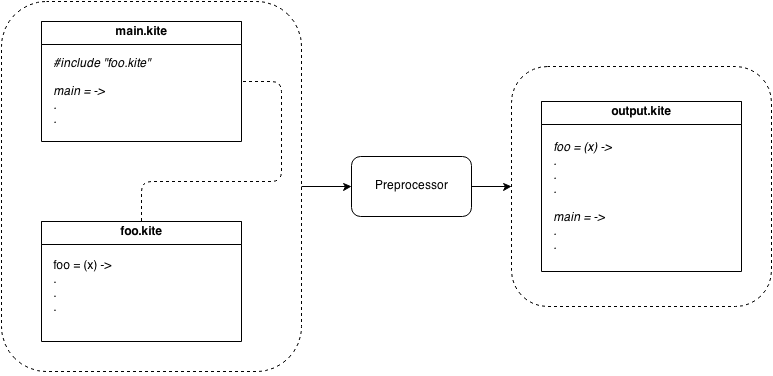
\includegraphics[scale=0.45]{images/preprocessor.png}
  \caption{Input and output of the Preprocessor}
\end{figure}

The nature of the preprocessor is quite simple, as the only task it
simple textual substitution.

\subsection{Lexical analysis}
The lexical analyzer, or just \emph{lexer}, is a central part of most
compilers. It has the important task of processing some input and
converting it to known, referencable tokens. This process is commonly
known as \emph{tokenization}.

Most lexers are quite simple, as they simply make tokens by matching the input with regular languages and classify the substrings according to these. Thus lexers do not perform any complex tasks - this is reserved for the parser and analyzer, which we will describe in the following.


\subsection{Parser}
The parser takes the list of tokens from the lexer and based on a
language grammar, it builds a corresponding data structure, namely the
parse tree. In the process it checks that that the input is
syntactically correct. Therefore, this process is also called syntactic
analysis.

In the cases know to us (Yacc, Happy, ANTLR), parser-generators make use of \emph{Context-Free Grammars} (CFG), and thus we have to define our desired syntax as a CFG.

The parser should rule out code containing syntactical errors, especially typos, which are likely to occur without a good IDE\footnote{IDE is short for Integrated Development Environment, which, among other features, often has good auto-completion, thus making typos much less likely.}.

\subsection{Desugar}
In order to make the language more convenient to write, we have made syntactic sugar and will introduce a desugaring module. This will take specific syntactic constructs and convert them into their more basic elements.

\subsection{Analyzer}
The analyzer will traverse the parse tree and perform \emph{typechecking} and look for calls to undefined functions. The analyser should spot almost all remaining incorrect code. Thus the output should be able to be executed without errors due to incorrect types, typos or the usage of undeclared variables.

The analyzer cannot, however, determine whether a program will yield the expected results or even if it will ever terminate.


\subsection{Optimizer}
The optimizer traverses the analysed parse tree and filters out unused functions. 
TODO: In implementation, mention that it does this by starting in the declaration of main, and keeps the actually applied functions, thus filtering out the unused functions and thereby reducing the size of the emitted code. 


\subsection{Code generation}
The code generator will take a representation of the
parse tree, the output of the parser, and generate code
accordingly. TODO: Inital, not done.
